\documentclass[tikz,border=5pt]{standalone}
\usepackage[T1]{fontenc}
\usepackage{lmodern,amsmath,amssymb}
\usetikzlibrary{arrows.meta,calc,positioning,fit,backgrounds,shapes.geometric,matrix,decorations.pathreplacing,patterns}
\definecolor{ink}{gray}{0.08}
\definecolor{wash}{gray}{0.965}
\definecolor{soft}{gray}{0.45}
\tikzset{box/.style={draw=ink,line width=.65pt,fill=white,align=center,inner sep=4pt,outer sep=0pt,font=\small},flow/.style={draw=ink,line width=.65pt,-{Latex[length=1.8mm,width=1.3mm]},rounded corners=2pt},annotation/.style={font=\scriptsize,text=soft,align=center},groupbox/.style={draw=soft,dashed,line width=.45pt,fill=wash}}
\begin{document}
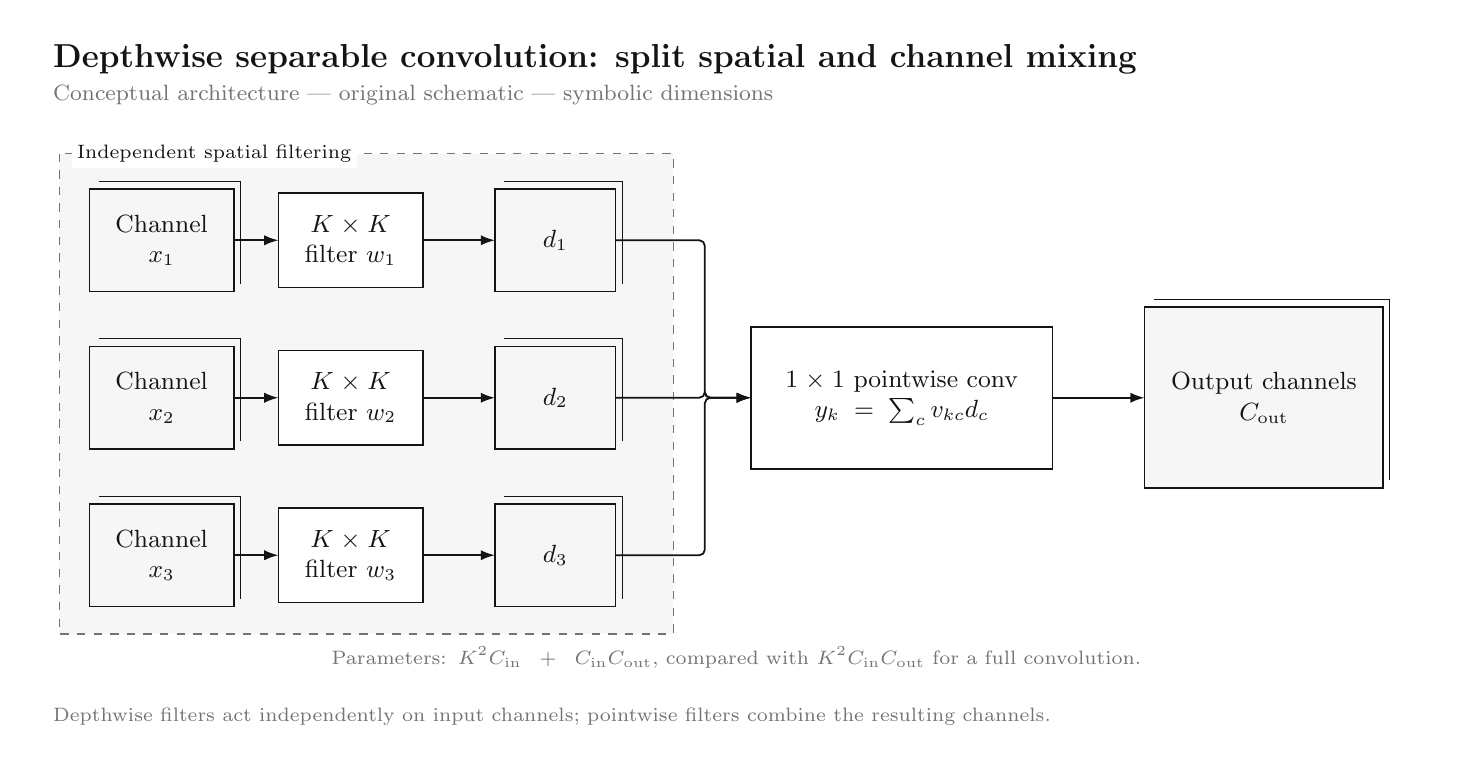
\begin{tikzpicture}[x=1cm,y=-1cm,font=\rmfamily,text=ink]

\path[use as bounding box] (0,0) rectangle (18,9);
\node[anchor=west,font=\large\bfseries] at (.2,.4) {Depthwise separable convolution: split spatial and channel mixing};
\node[anchor=west,font=\footnotesize,text=soft] at (.2,.85) {Conceptual architecture | original schematic | symbolic dimensions};
\begin{pgfonlayer}{background}
\draw[groupbox] (0.4,1.6) rectangle (8.2,7.699999999999999);
\node[anchor=west,font=\scriptsize,fill=white,inner sep=2pt] at (0.55,1.6) {Independent spatial filtering};
\end{pgfonlayer}
\node[box,fill=wash,minimum width=1.8cm,minimum height=1.3cm,text width=1.55cm] (x1) at (1.7,2.7) {Channel $x_1$};
\draw[ink,line width=.4pt] (0.8999999999999999,1.9500000000000002) -- (2.7,1.9500000000000002) -- (2.7,3.25);
\node[box,minimum width=1.8cm,minimum height=1.2cm,text width=1.55cm] (k1) at (4.1,2.7) {$K\times K$\\filter $w_1$};
\node[box,fill=wash,minimum width=1.5cm,minimum height=1.3cm,text width=1.25cm] (d1) at (6.7,2.7) {$d_1$};
\draw[ink,line width=.4pt] (6.05,1.9500000000000002) -- (7.55,1.9500000000000002) -- (7.55,3.25);
\node[box,fill=wash,minimum width=1.8cm,minimum height=1.3cm,text width=1.55cm] (x2) at (1.7,4.7) {Channel $x_2$};
\draw[ink,line width=.4pt] (0.8999999999999999,3.9499999999999997) -- (2.7,3.9499999999999997) -- (2.7,5.250000000000001);
\node[box,minimum width=1.8cm,minimum height=1.2cm,text width=1.55cm] (k2) at (4.1,4.7) {$K\times K$\\filter $w_2$};
\node[box,fill=wash,minimum width=1.5cm,minimum height=1.3cm,text width=1.25cm] (d2) at (6.7,4.7) {$d_2$};
\draw[ink,line width=.4pt] (6.05,3.9499999999999997) -- (7.55,3.9499999999999997) -- (7.55,5.250000000000001);
\node[box,fill=wash,minimum width=1.8cm,minimum height=1.3cm,text width=1.55cm] (x3) at (1.7,6.7) {Channel $x_3$};
\draw[ink,line width=.4pt] (0.8999999999999999,5.95) -- (2.7,5.95) -- (2.7,7.250000000000001);
\node[box,minimum width=1.8cm,minimum height=1.2cm,text width=1.55cm] (k3) at (4.1,6.7) {$K\times K$\\filter $w_3$};
\node[box,fill=wash,minimum width=1.5cm,minimum height=1.3cm,text width=1.25cm] (d3) at (6.7,6.7) {$d_3$};
\draw[ink,line width=.4pt] (6.05,5.95) -- (7.55,5.95) -- (7.55,7.250000000000001);
\node[box,minimum width=3.8cm,minimum height=1.8cm,text width=3.55cm] (pw) at (11.1,4.7) {$1\times1$ pointwise conv\\$y_k=\sum_c v_{kc}d_c$};
\node[box,fill=wash,minimum width=3.0cm,minimum height=2.3cm,text width=2.75cm] (y) at (15.7,4.7) {Output channels\\$C_{\rm out}$};
\draw[ink,line width=.4pt] (14.299999999999999,3.45) -- (17.3,3.45) -- (17.3,5.75);
\begin{pgfonlayer}{background}
\draw[flow] (x1.east) -- (k1.west);
\draw[flow] (k1.east) -- (d1.west);
\draw[flow] (x2.east) -- (k2.west);
\draw[flow] (k2.east) -- (d2.west);
\draw[flow] (x3.east) -- (k3.west);
\draw[flow] (k3.east) -- (d3.west);
\draw[flow] (d1.east) -- (8.6,2.7) -- (8.6,4.7) -- (pw.west);
\draw[flow] (d2.east) -- (8.6,4.7) -- (8.6,4.7) -- (pw.west);
\draw[flow] (d3.east) -- (8.6,6.7) -- (8.6,4.7) -- (pw.west);
\draw[flow] (pw.east) -- (y.west);
\end{pgfonlayer}
\node[annotation,text width=16cm] at (9,8.0) {Parameters: $K^2C_{\rm in}+C_{\rm in}C_{\rm out}$, compared with $K^2C_{\rm in}C_{\rm out}$ for a full convolution.};
\node[anchor=west,align=left,font=\scriptsize,text=soft,text width=17.6cm] at (.2,8.75) {Depthwise filters act independently on input channels; pointwise filters combine the resulting channels.};
\end{tikzpicture}
\end{document}
